\section{湍流预混火焰}
\subsection{概述}
\subsection{一些应用}
\subsubsection{电火花点火发动机}
\subsubsection{燃气轮机}
\subsubsection{工业气体燃烧器}
\subsection{湍流火焰传播速度定义}
\begin{equation}
    S_\mathrm{t} = \frac{\dot{m}}{\overline{A} \rho_u}
\end{equation}其中\(\dot{m}\)是反应物的质量流量;\(\rho_\mathrm{u}\)是未燃气体密度;\(\overline{A}\)是时间平滑后的火焰面积。这一速度也被称为\textbf{通用消耗速度}。
\subsection{湍流预混火焰结构}
\subsubsection{实验观察}
\begin{figure}[H]
    \centering
    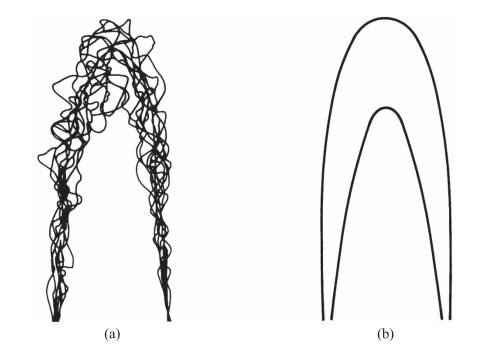
\includegraphics[width=.3\textwidth]{img/turb_prem_image.png}
\end{figure}
我们称这一有明显厚度的反应区为\textbf{湍流火焰刷}。瞬时的图像说明,实际的反应区像层流预混火焰一样,相对是很薄的。这些反应区有时也称为\textbf{层流火焰片}。

\subsubsection{三种火焰模式}

\textbf{模型判据}:

\begin{itemize}
    \item 褶皱层流火焰模式:\(\delta_L\le \mathcal{l}_\mathrm{K}\):威廉斯-克里莫夫(Williams-Klimov)判据。
    \item 分布反应模式:反应区内的输运现象就不仅受分子运动的控制,同时也受湍流运动的控制,或者至少要受湍流运动的影响。\(\delta_L > \mathcal{l}_0\):丹姆克尔(Damköhler)判据。
    \item 漩涡小火焰模式:\(\mathcal{l}_0 > \delta_\mathrm{L} > \mathcal{l}_\mathrm{K}\)。
\end{itemize}

利用\(\mathcal{l}_\mathrm{K}\delta_\mathrm{L}\)和\(\mathcal{l}_0/\delta_\mathrm{L}\),湍流雷诺数\(Re_{t_0}\)和丹姆克尔数\(Da\),来进行分析。

\textbf{丹姆克尔数}:

\begin{equation}
    Da = \frac{\tau_\mathrm{flow}}{\tau_\mathrm{chem}}
\end{equation}

是流体的流动特征时间或混合时间与化学特征时间的比值。

流体中最大漩涡的存在时间:\(\tau_\mathrm{flow}\equiv \mathcal{l}_0/v_\mathrm{rms}'\)和化学特征时间\(\tau_\mathrm{chem}\equiv \delta_L/S_L\)。这两个数字的比值就是丹姆克尔数。

\begin{equation}
    Da = \frac{\mathcal{l}_0/v_\mathrm{rms}'}{\delta_L / S_L} = \frac{\mathcal{l}_0}{\delta_L} \frac{S_L}{v_\mathrm{rms}'}
\end{equation}
\textbf{快速化学反应模式}:化学反应速率比流体的混合速度快时,\(Da\ge 1\)。

\begin{figure}[H]
    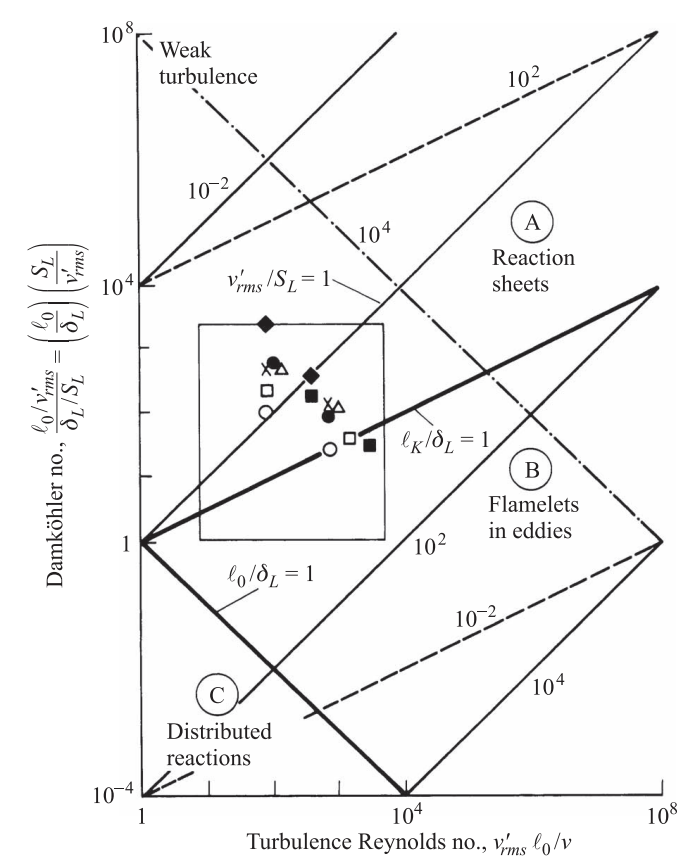
\includegraphics[width=.3\textwidth]{img/turb_premixed_type.png}
\end{figure}

\begin{enumerate}
    \item 两根粗线把空间分成了三个区域,代表了湍流火焰的三种模式;
    \item 两根粗线分别代表了\textit{层流火焰厚度}等于\textit{湍流的积分尺度}和\textit{层流火焰厚度}等于\textit{柯尔莫哥洛夫微尺度}的时候;
    \item 在\(\mathcal{l}_K/\delta_L=1\)的粗线上方,反应发生在很薄的片内,也就是\textit{褶皱层流火焰模式};
    \item 在\(\mathcal{l}_0/\delta_L=1\)的粗线下方,反应发生在空间分布相对较厚的区域内,也就是\textit{分布反应模式};
    \item 两条粗线中间就是\textit{漩涡小火焰模式}。
\end{enumerate}

\subsection{褶皱层流火焰模式}
湍流唯一的作用就是使得火焰面褶皱,从而增大火焰面积。湍流火焰传播速度与层流火焰传播速度的比值就相当于褶皱火焰面积与时间平均火焰面积之比。
\begin{equation}
    S_t/S_L = A_\mathrm{flamelets}/\overline{A}
\end{equation}

\begin{enumerate}
    \item 丹姆克尔模型:
    
    \(S_{t}/S_{L}=1+\nu_{m s}^{\prime}/S_{L}\);
    \item 克拉文和威廉斯模型:
    
    \(S_{t}/S_{L}=\Big\{0.5\Big[1+\Big(1+8C v_\mathrm{rms}^{\prime2}/S_{L}^{2}\Big)^{1/2}\,\Big]\Big\}^{1/2}\);其中\(C\)是接近1的常数,如果\(v_\mathrm{rms}'/S_L\)比较小,那么这个式子可以被简化为:\(S_{t}/S_{L}=1+C v_\mathrm{rms}^{\prime2}/S_{L}^{2}\);
    \item 克里莫夫模型:
    
    \(S_{t}/S_{L}=3.5(v_\mathrm{rms}^{\prime}/S_{L})^{0.7}\)。这个式子在\(v_\mathrm{rms}'/S_L\gg 1\)时成立。

    \item 三个模型的\(S_t/S_L\)都只与\(v_\mathrm{rms}'/S_L\)有关。
\end{enumerate}

\subsubsection{分布反应模式}
\textit{这个模式在实际的设备中很难实现}
\begin{enumerate}
    \item \(\mathcal{l}_0/\delta_L\)且\(Da<1\)的时候火焰进入分布反应模式;
    \item \(\mathcal{l}\)很小,但是\(v_\mathrm{rms}'\)很大,也就是流道小,速度大;
    \item 压力损失大;
    \item 火焰难以维持。
\end{enumerate}

这个东西很难求解。

\begin{figure}[H]
    \begin{subfigure}[t]{.15\textwidth}
        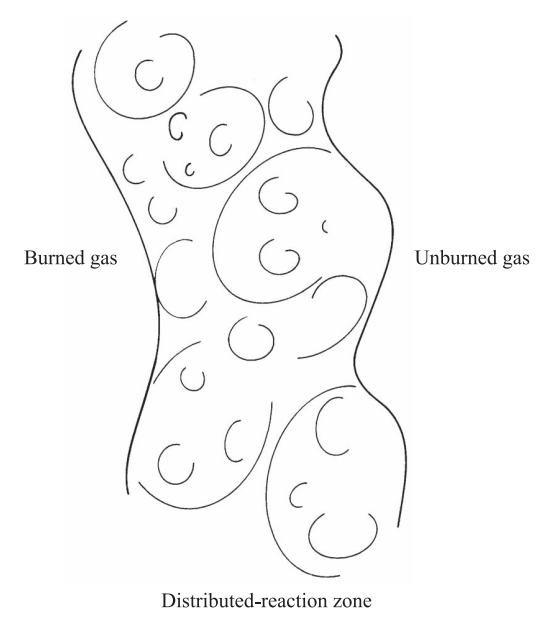
\includegraphics[width=.99\textwidth]{img/distributed_reaction.png}
        \caption{湍流火焰在分布反应模式下传播的概念图}
    \end{subfigure}
    \begin{subfigure}[t]{.15\textwidth}
        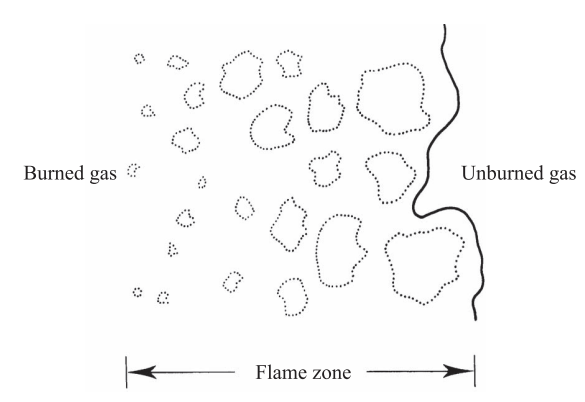
\includegraphics[width=.99\textwidth]{img/flamelet_in_eddies.png}
        \caption{湍流火焰在漩涡内小火焰模式中传播的概念图}
    \end{subfigure}
\end{figure}

\subsection{漩涡内小火焰模式}
\begin{itemize}
    \item 中等大小的\(Da\)和很高的湍流强度\(v_\mathrm{rms}'/S_L\gg 1\);
    \item 电火花点火发动机就是处于这一范围。
\end{itemize}

\textbf{旋涡破碎模型的理论}:
\begin{enumerate}
    \item 燃烧速率取决于未燃气团破碎成更小微团的速率;
    \item 破碎使得未燃混合物与已燃热延期之间有足够的界面进行反应;
    \item 完全由湍流混合速度控制着燃烧过程。
\end{enumerate}

单位体积燃料的质量燃烧速率为:
\begin{equation}
    \overline{\dot{m}}_F''' = -\rho C_F Y_{F, rms}' \epsilon_0 / (3 v_{rms}'^2 / 2)
\end{equation}\(\epsilon_0\)时湍流耗散率,如果我们认为湍流个像同性,将所有常数归入\(C_F\),可以得到:
\begin{equation}
    \overline{\dot{m}}_F''' = -\rho c_F Y_{F,rms}' v_{rms}' / \mathcal{l}_0
\end{equation}

\subsection{火焰稳定}

\subsubsection{旁路喷嘴}
\begin{figure}[H]
    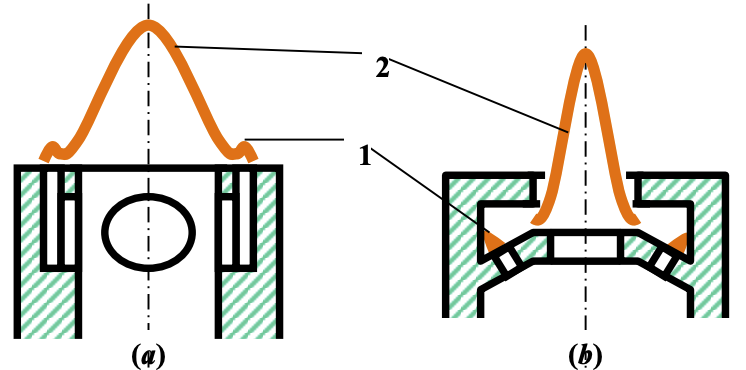
\includegraphics[width=.3\textwidth]{img/zhiban.png}
\end{figure}
\subsubsection{燃烧器耐火碹口}
\begin{figure}[H]
    \centering
    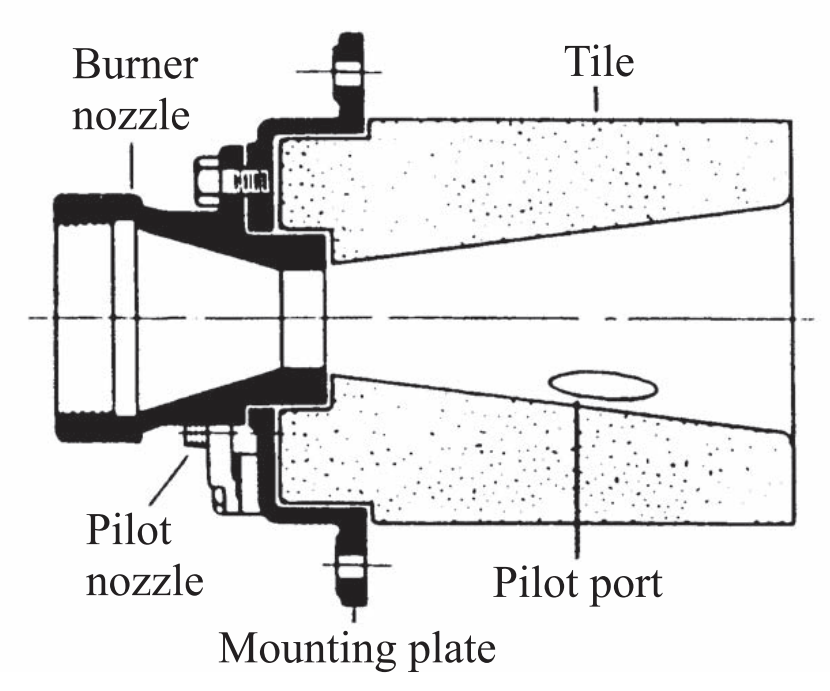
\includegraphics[width=.3\textwidth]{img/tiles.png}
\end{figure}

\begin{enumerate}
    \item 火焰被稳定在一个耐火的通道;
    \item 碹口形成绝热边界,将热量辐射回火焰中,火焰温度接近绝热燃烧温度,这样能提高湍流燃烧速度;
    \item 碹口的扩张叫很大,使得边界层可能分离而在碹口内形成回流区,使得高温烟气回流到上游,进一步促进未燃混合物着火。
\end{enumerate}
\subsubsection{钝体}
在钝体后面形成强烈的回流区,下图亮区所示。回流区由均匀的接近绝热燃烧温度的燃烧产物组成。火焰稳定点接近稳燃器的边缘。
\subsubsection{旋流和射流诱导回流流动}
在来流中运用旋流元件或者在燃烧空间中引入一股射流都可以形成回流区,使火焰稳定。
\subsubsection{其他}
\begin{enumerate}
    \item 突扩燃烧室:在突扩处形成回流区;
    \item 壁面凹槽:在凹槽处产生回流区;
    \item 逆向射流稳定火焰:在高速可燃气流中射入一股逆向射流(空气或混合气)来稳定火焰的
    \begin{enumerate}
        \item 在主流中射入一股逆向射流后,射流将逐渐减速,直到在射流顶部形成一个滞止区,从这里开始,射流部分结构特性象一个钝体,在滞止区与喷口之间形成环流区和回流区;
        \item 滞止区里主流及逆向射流的混合气在回流的炽热气体的点燃下,成为一个稳定的点火区,初始火焰在这里产生并向外传播,在主流的作用下,火焰呈抛物面形。
    \end{enumerate}
\end{enumerate}
